%===============================================================================
% Zentrale Layout-Angaben und Befehle
%===============================================================================
%
% F???r bessere Sicht von falschen Umbr???chen die Option draft benutzen.
% Dadurch k???nnen aber die eingebundenen Bilder nicht sichtbar sein.
\documentclass[a4paper, 12pt]{article}
%
% Hier zun???chst die ben???tigten Packages
%\usepackage[utf-8]{inputenc}
\usepackage{fancyhdr}
\usepackage{pifont}
\usepackage{fontspec}
\usepackage{xunicode}
%\usepackage{ae}
\usepackage{listings}
\usepackage{color}
\usepackage[rgb]{xcolor}
\usepackage{listings}
\usepackage{newfloat,caption}
\usepackage{subcaption}
\usepackage{wrapfig}
\usepackage[printonlyused]{acronym}
\usepackage[hyphens]{url}
\usepackage[dirty=*]{gitinfo2}
\usepackage[pdfauthor={Florian Beetz},
            pdftitle={Beyond REST: GraphQL as an Alternative for Microservice APIs},
            pdfcreator={Build using git hash \gitHash\gitDirty}]{hyperref}
\usepackage{booktabs}
\usepackage{amssymb}
%
% Einbindung des Grafik-Pakets
%\ifx\pdfoutput\undefined
%	\usepackage[dvips]{graphicx}
%\else
%	\usepackage[pdftex]{graphicx}
%\pdfcompresslevel=9
%\pdfpageheight=297mm
%\pdfpagewidth=210mm
%\fi
\usepackage{graphicx}
\usepackage{enumitem}
\usepackage{csquotes}
%
\usepackage{tikz}
\usetikzlibrary{positioning,arrows,fit,calc,shapes,shapes.multipart,shapes.geometric,patterns}
\pgfdeclarelayer{background}
\pgfdeclarelayer{foreground}
\pgfsetlayers{background,main,foreground}
%
% Page-Layout
\setlength\headheight{14pt}
\setlength\topmargin{-15,4mm}
\setlength\oddsidemargin{-0,4mm}
\setlength\evensidemargin{-0,4mm}
\setlength\textwidth{160mm}
\setlength\textheight{252mm}
%
% Absatzeinstellungen
\setlength\parindent{0mm}
\setlength\parskip{2ex}
%
% Kopf- und Fusszeile
\pagestyle{fancy}
\fancyhf{} % alles l�schen
\fancyhead[LO]{\footnotesize\sc\nouppercase{\leftmark}}
\fancyfoot[LO]{\footnotesize\sc Lehrstuhl für Praktische Informatik}
\fancyfoot[RO]{\thepage}
\renewcommand{\headrulewidth}{0pt}
\renewcommand{\footrulewidth}{0pt}
%
% Bessere Fehlermeldungen
\errorcontextlines=999
%
% Anweisung zur Erstellung der Titelseite
% #1 Bachelorarbeit || Masterarbeit
% #2 = Studiengang
% #3 = Titel der Arbeit
% #4 = Autor
% #5 = Abgabedatum
\renewcommand{\maketitle}[5]
{
\pagenumbering{Alph}
\begin{titlepage}
\centering
\begin{minipage}[t]{16cm}
\begin{minipage}{3cm}
    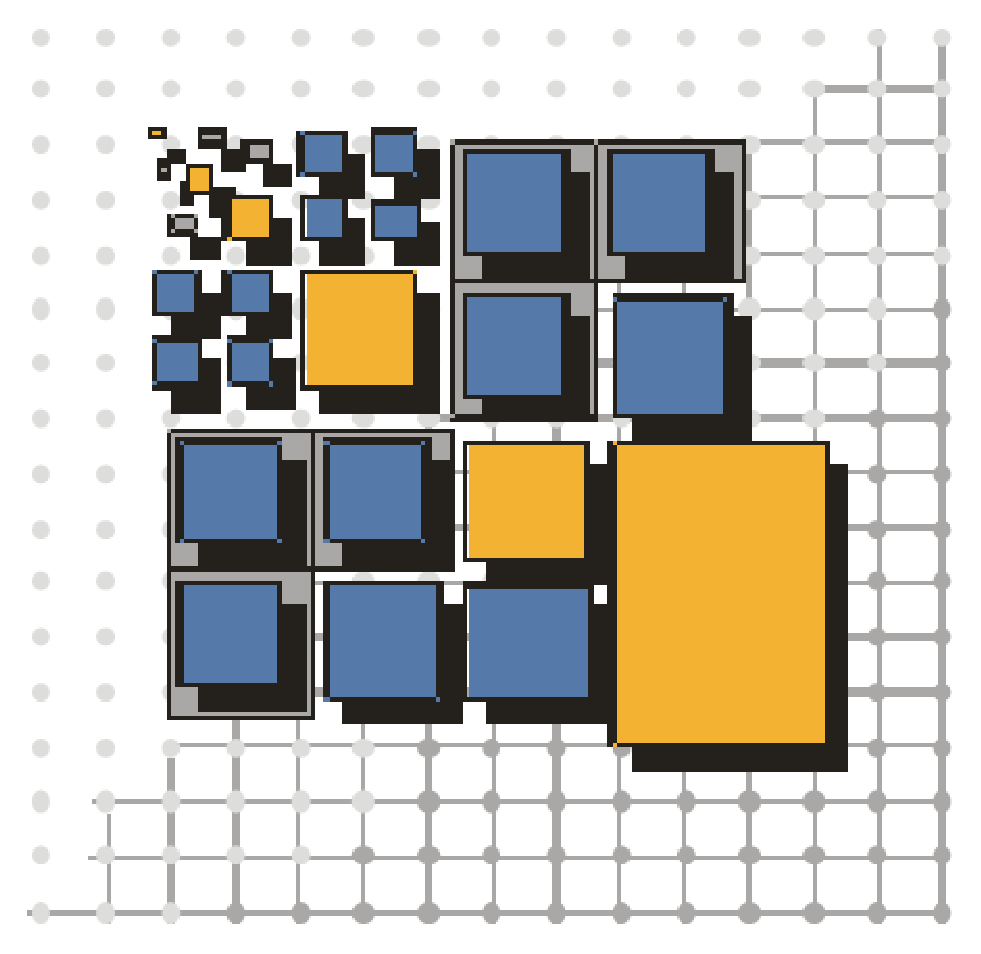
\includegraphics[height=26mm]{includes/vs-logo}
\end{minipage}
\hfill
\begin{minipage}{9cm}
  \centering
    Otto-Friedrich-Universität Bamberg\\[12pt]
    {\Large Lehrstuhl für Praktische Informatik}
\end{minipage}
\hfill
\begin{minipage}{3cm}
    
\includegraphics[height=26mm]{includes/UB-Logo-neu_blau-cmyk}
\end{minipage}
\end{minipage}\\[130pt]
{\LARGE #1}\\[24pt]
im Studiengang #2\\
der Fakultät Wirtschaftsinformatik und Angewandte Informatik\\
der Otto-Friedrich-Universität Bamberg\\[90pt]
Zum Thema:\\[24pt]
{\Huge #3}\\[60pt]
\vfill
\begin{minipage}{\textwidth}
\center
Vorgelegt von:\\
{\Large #4\\[12pt]}
Themensteller:\\
Prof. Dr. Guido Wirtz\\[12pt]
Abgabedatum:\\
#5\\
\end{minipage}
\end{titlepage}
}
%
% Anweisung zur Erstellung der Eigenst�ndigkeitserkl�rung
% #1 = Typ der Arbeit
% #2 = Datum
% #3 = Vorname Name
\newcommand{\makedeclaration}[3]
{
	\fancyhead[LO]{\footnotesize\sc\nouppercase{Eigenständigkeitserklärung}}
	%
			\vspace*{18cm}
			Ich erkläre hiermit gemäß § 9 Abs. 12 APO, dass ich die vorstehende #1 selbstständig verfasst 
      und keine anderen als die angegebenen Quellen und Hilfsmittel benutzt habe.\\
			\vspace*{1cm}
			
			Bamberg, den #2 \hspace{5cm} #3
	%
}
%
% Wird f�r Hintergrund von Codelistings ben�tigt
\definecolor{hellgrau}{gray}{0.9}
%
% Einstellungen f�r Java-Code
\lstdefinestyle{javaStyle}{%
  basicstyle=\small,%
  backgroundcolor=\color{hellgrau},%
  keywordstyle=\bfseries,%
  showstringspaces=false,%
  language=Java,%
  numbers=left,%
  numberstyle=\tiny,%
  stepnumber=1,%
  numbersep=5pt,%
  extendedchars=true,%
  xleftmargin=2em,%
  lineskip=-1pt,%
  breaklines%
}
%
% neues environment f�r Java-Sourcecode
% #1 = "caption={Hier eigene �berschrift}, label={Hier eigenes Label}"
\lstnewenvironment{javacode}[1][]{%
\lstset{style=javaStyle,#1}%
}{}
%
% Befehl zum Einbinden von Java-Sourcecode aus Datei
% #1 = Dateiname relativ zu src-Verzeichnis
% #2 = �berschrift
% #3 = Label
\newcommand{\javafile}[3]{%
   \lstinputlisting[%
     caption={#2},%
     label={#3},%
     style=javaStyle]{src/#1}%
}
%
% Einbindung eines Bildes
% #1 = label f�r \ref-Verweise
% #2 = Name des Bildes ohne Endung relativ zu images-Verzeichnis
% #3 = Beschriftung
% #4 = Breite des Bildes im Dokument in cm
\newcommand{\bild}[4]{%
  \begin{figure}[htb]%
    \begin{center}%
      \includegraphics[width=#4cm]{images/#2}%
      \vskip -0.3cm%
      \caption{#3}%
      \vskip -0,2cm%
      \label{#1}%
    \end{center}%
  \end{figure}%
}
%
% Umgebung f�r Fliesstext um Grafik
% #1 = Ausrichtung: r, l, i, ...
% #2 = Breite des Bildes in cm
% #3 = Name des Bildes ohne Endung relativ zu images-Verzeichnis
% #4 = Beschriftung
% #5 = label f�r \ref-Verweise
\newcommand{\fliesstext}[5]{%
\begin{wrapfigure}{#1}{#2cm}%
\includegraphics[width=#2cm]{images/#3}%
\caption{#4}%
\label{#5}%
\end{wrapfigure}%
}
%%% Local Variables:
%%% mode: latex
%%% TeX-master: t
%%% End:

\definecolor{theme1}{HTML}{A6325C}
\definecolor{theme2}{HTML}{0477BF}
\definecolor{theme3}{HTML}{03A64A}
\definecolor{theme4}{HTML}{F29F05}
\definecolor{theme5}{HTML}{F24141}


\definecolor{solarized-orange}{HTML}{cb4b16}
\definecolor{solarized-cyan}{HTML}{2aa198}
\definecolor{solarized-base1}{HTML}{93a1a1}
\definecolor{solarized-green}{HTML}{859900}
\definecolor{solarized-magenta}{HTML}{d33682}
\definecolor{solarized-yellow}{HTML}{b58900}
\definecolor{solarized-blue}{HTML}{268bd2}



\lstset{
  basicstyle=\ttfamily\footnotesize,
  numbers=left,
  numbersep=5pt,
  numberstyle=\ttfamily\footnotesize\textcolor{solarized-base1},
  keywordstyle=\textcolor{solarized-orange},
  stringstyle=\textcolor{solarized-green},
  commentstyle=\textcolor{solarized-base1},
  showstringspaces=false,
  xleftmargin=5ex,
  captionpos=b,
  escapeinside={(*}{*)}
}
\lstdefinelanguage{http}{
  keywords={Host, Accept, Server, Content, Type, Length, ETag, If, Match},
  keywordstyle=\textbf,
  moredelim=[is][\bfseries]{[*}{*]}
}
\lstdefinelanguage{graphql}{
  keywords={query, mutation, subscription, {...}, on, true, false, null},
  morestring=[b]",
  comment=[l]{\#},
  literate=%
    *{0}{{{\textcolor{solarized-magenta}0}}}1
    {1}{{{\textcolor{solarized-magenta}1}}}1
    {2}{{{\textcolor{solarized-magenta}2}}}1
    {3}{{{\textcolor{solarized-magenta}3}}}1
    {4}{{{\textcolor{solarized-magenta}4}}}1
    {5}{{{\textcolor{solarized-magenta}5}}}1
    {6}{{{\textcolor{solarized-magenta}6}}}1
    {7}{{{\textcolor{solarized-magenta}7}}}1
    {8}{{{\textcolor{solarized-magenta}8}}}1
    {9}{{{\textcolor{solarized-magenta}9}}}1
    {...}{{{\textcolor{solarized-orange}{...}}}}2
    {person}{{\textcolor{solarized-cyan}{person}}}5
    {personID}{{\textcolor{solarized-cyan}{personID}}}7
    {name}{{\textcolor{solarized-cyan}{name}}}3
    {filmConnection}{{\textcolor{solarized-cyan}{filmConnection}}}{12}
    {films}{{\textcolor{solarized-cyan}{films}}}4
    {title}{{\textcolor{solarized-cyan}{title}}}4
    {market}{{\textcolor{solarized-cyan}{market}}}5
    {addReview}{{\textcolor{solarized-cyan}{addReview}}}8
    {filmId}{{\textcolor{solarized-cyan}{filmId}}}5
    {rating}{{\textcolor{solarized-cyan}{rating}}}5
    {comment}{{\textcolor{solarized-cyan}{comment}}}6
    {success}{{\textcolor{solarized-cyan}{success}}}6
    {review}{{\textcolor{solarized-cyan}{review}}}5
    {reviews}{{\textcolor{solarized-cyan}{reviews}}}6
    {id}{{\textcolor{solarized-cyan}{id}}}1
    {stellarObjects}{{\textcolor{solarized-cyan}{stellarObjects}}}{13}
    {position}{{\textcolor{solarized-cyan}{position}}}{7}
    {inhabitable}{{\textcolor{solarized-cyan}{inhabitable}}}{10}
    {Planet}{{\textcolor{solarized-yellow}{Planet}}}{5}
    {\$experimentalFeatures}{{\textcolor{solarized-blue}{\$experimentalFeatures}}}{19}
    {Boolean}{{\textcolor{solarized-yellow}{Boolean}}}{6}
    {regularField}{{\textcolor{solarized-cyan}{regularField}}}{11}
    {experimentalField}{{\textcolor{solarized-cyan}{experimentalField}}}{15}
    {@include}{{\textcolor{solarized-magenta}{@include}}}{7}
    {if}{{\textcolor{solarized-cyan}{if}}}{2}
    {me}{{\textcolor{solarized-cyan}{me}}}{2}
    {body}{{\textcolor{solarized-cyan}{body}}}{4}
    {product}{{\textcolor{solarized-cyan}{product}}}{7}
    {price}{{\textcolor{solarized-cyan}{price}}}{5}
}

\lstdefinelanguage{json}{
  morestring=[b]",
  literate=%
    *{0}{{{\textcolor{solarized-magenta}0}}}1
    {1}{{{\textcolor{solarized-magenta}1}}}1
    {2}{{{\textcolor{solarized-magenta}2}}}1
    {3}{{{\textcolor{solarized-magenta}3}}}1
    {4}{{{\textcolor{solarized-magenta}4}}}1
    {5}{{{\textcolor{solarized-magenta}5}}}1
    {6}{{{\textcolor{solarized-magenta}6}}}1
    {7}{{{\textcolor{solarized-magenta}7}}}1
    {8}{{{\textcolor{solarized-magenta}8}}}1
    {9}{{{\textcolor{solarized-magenta}9}}}1
    {"data"}{{\textcolor{solarized-cyan}{"data"}}}5
    {"person"}{{\textcolor{solarized-cyan}{"person"}}}7
    {"name"}{{\textcolor{solarized-cyan}{"name"}}}5
    {"filmConnection"}{{\textcolor{solarized-cyan}{"filmConnection"}}}{14}
    {"films"}{{\textcolor{solarized-cyan}{"films"}}}6
    {"title"}{{\textcolor{solarized-cyan}{"title"}}}6
    {"boolean"}{{\textcolor{solarized-cyan}{"boolean"}}}8
    {"number"}{{\textcolor{solarized-cyan}{"number"}}}7
    {"string"}{{\textcolor{solarized-cyan}{"string"}}}7
    {"array"}{{\textcolor{solarized-cyan}{"array"}}}6
    {"query"}{{\textcolor{solarized-cyan}{"query"}}}6
    {"errors"}{{\textcolor{solarized-cyan}{"errors"}}}7
    {"extensions"}{{\textcolor{solarized-cyan}{"extensions"}}}{11}
    {"someId"}{{\textcolor{solarized-cyan}{"someId"}}}7
    {"variables"}{{\textcolor{solarized-cyan}{"variables"}}}{10}
    {"nullValue"}{{\textcolor{solarized-cyan}{"nullValue"}}}{10}
    {true}{{\textcolor{solarized-orange}{true}}}4
    {false}{{\textcolor{solarized-orange}{false}}}5
    {null}{{\textcolor{solarized-orange}{null}}}4
}
\lstdefinelanguage{yaml}{
  keywords={true,false,null,y,n},
  sensitive=false,
  comment=[l]{\#},
  morecomment=[s]{/*}{*/},
  moredelim=[l][\color{orange}]{\&},
  moredelim=[l][\color{magenta}]{*},
  morestring=[b]',
  morestring=[b]",
  literate =    {=}{{\textcolor{black}{=}}}1
                {"}{{\textcolor{black}{"}}}1
                {labels}{{\textcolor{solarized-cyan}{labels}}}6
                {true}{{\textcolor{solarized-orange}{true}}}4
                {PathPrefix}{{\textcolor{solarized-magenta}{PathPrefix}}}{9}
                {`/inventory/`}{{\textcolor{solarized-green}{`/inventory/`}}}{12}
                {web}{{\textcolor{solarized-green}{web}}}{3}
}

\lstdefinelanguage{graphqls}{
  keywords={query, mutation, type, schema, enum, interface, implements, union, input, directive, on, extend},
  comment=[l]{\#},
  morestring=[b]",
  literate=%
    *{0}{{{\textcolor{solarized-magenta}0}}}1
    {1}{{{\textcolor{solarized-magenta}1}}}1
    {2}{{{\textcolor{solarized-magenta}2}}}1
    {3}{{{\textcolor{solarized-magenta}3}}}1
    {4}{{{\textcolor{solarized-magenta}4}}}1
    {5}{{{\textcolor{solarized-magenta}5}}}1
    {6}{{{\textcolor{solarized-magenta}6}}}1
    {7}{{{\textcolor{solarized-magenta}7}}}1
    {8}{{{\textcolor{solarized-magenta}8}}}1
    {9}{{{\textcolor{solarized-magenta}9}}}1
    {@}{{{\textcolor{solarized-magenta}@}}}1
    {key}{{{\textcolor{solarized-magenta}{key}}}}3
    {skip}{{{\textcolor{solarized-magenta}{skip}}}}4
    {deprecated}{{{\textcolor{solarized-magenta}{deprecated}}}}{9}
    {external}{{{\textcolor{solarized-magenta}{external}}}}{7}
    {provides}{{{\textcolor{solarized-magenta}{provides}}}}{7}
    {requires}{{{\textcolor{solarized-magenta}{requires}}}}{7}
    {name}{{\textcolor{solarized-cyan}{name}}}4
    {appearsIn}{{\textcolor{solarized-cyan}{appearsIn}}}8
    {id}{{\textcolor{solarized-cyan}{id}}}2
    {length}{{\textcolor{solarized-cyan}{length}}}6
    {hero}{{\textcolor{solarized-cyan}{hero}}}4
    {droid}{{\textcolor{solarized-cyan}{droid}}}5
    {unit}{{\textcolor{solarized-cyan}{unit}}}4
    {episode}{{\textcolor{solarized-cyan}{episode}}}7
    {~query}{{\textcolor{solarized-cyan}{query}}}5
    {~mutation}{{\textcolor{solarized-cyan}{mutation}}}8
    {episode}{{\textcolor{solarized-cyan}{episode}}}7
    {position}{{\textcolor{solarized-cyan}{position}}}8
    {inhabitable}{{\textcolor{solarized-cyan}{inhabitable}}}{11}
    {ownerId}{{\textcolor{solarized-cyan}{ownerId}}}{7}
    {success}{{\textcolor{solarized-cyan}{success}}}{7}
    {vehicle}{{\textcolor{solarized-cyan}{vehicle}}}{7}
    {vehicleType}{{\textcolor{solarized-cyan}{vehicleType}}}{11}
    {createVehicle}{{\textcolor{solarized-cyan}{createVehicle}}}{13}
    {newField}{{\textcolor{solarized-cyan}{newField}}}{8}
    {oldField}{{\textcolor{solarized-cyan}{oldField}}}{8}
    {if}{{\textcolor{solarized-cyan}{if}}}{2}
    {reason}{{\textcolor{solarized-cyan}{reason}}}{6}
    {reviews}{{\textcolor{solarized-cyan}{reviews}}}{7}
    {recentPurchases}{{\textcolor{solarized-cyan}{recentPurchases}}}{14}
    {price}{{\textcolor{solarized-cyan}{price}}}{5}
    {body}{{\textcolor{solarized-cyan}{body}}}{4}
    {author}{{\textcolor{solarized-cyan}{author}}}{6}
    {product}{{\textcolor{solarized-cyan}{product}}}{7}
    {fields}{{\textcolor{solarized-cyan}{fields}}}{6}
    {me}{{\textcolor{solarized-cyan}{me}}}{2}
    {String}{{\textcolor{solarized-yellow}{String}}}6
    {ID}{{\textcolor{solarized-yellow}{ID}}}2
    {Float}{{\textcolor{solarized-yellow}{Float}}}5
    {Boolean}{{\textcolor{solarized-yellow}{Boolean}}}6
    {Episode}{{\textcolor{solarized-yellow}{Episode}}}7
    {LengthUnit}{{\textcolor{solarized-yellow}{LengthUnit}}}8
    {~Character}{{\textcolor{solarized-yellow}{Character}}}9
    {Droid}{{\textcolor{solarized-yellow}{Droid}}}5
    {Repulsorcraft}{{\textcolor{solarized-yellow}{Repulsorcraft}}}{13}
    {WheeledVehicle}{{\textcolor{solarized-yellow}{WheeledVehicle}}}{14}
    {~User}{{\textcolor{solarized-yellow}{User}}}{4}
    {~Product}{{\textcolor{solarized-yellow}{Product}}}{7}
    {~Review}{{\textcolor{solarized-yellow}{Review}}}{6}
    {~Query}{{\textcolor{solarized-yellow}{Query}}}5
    {~Mutation}{{\textcolor{solarized-yellow}{Mutation}}}8
    {~Starship}{{\textcolor{solarized-yellow}{Starship}}}8
    {~Vehicle}{{\textcolor{solarized-yellow}{Vehicle}}}7
    {~VehicleInput}{{\textcolor{solarized-yellow}{VehicleInput}}}{10}
    {~CreateVehicleResponse}{{\textcolor{solarized-yellow}{CreateVehicleResponse}}}{19}
}
\lstdefinelanguage{javascript}{
  keywords={const, new},
  morestring=[d]['],
  stringstyle=\textcolor{solarized-green},
}
%
\tikzset{
  >=stealth',
	every node/.style = {
		font = \sffamily
	}
}

\DeclareFloatingEnvironment[fileext=frm,placement={!ht},name=Listing,within=section]{listing}
